\documentclass{beamer}
\usepackage[utf8]{inputenc}
\usepackage[english]{babel}
\usepackage{wrapfig}
\usepackage{verbatim}

\title{Parallel(?) Tempering}
\author{Rômulo Cenci}
\date{\today}

\begin{document}

\frame{\titlepage}

\begin{frame}
  \frametitle{So.. Who am I?}
  \begin{itemize}
  \item Universidade Federal de Santa Catarina - Florianópolis, Brazil.
  \item Advisor: Lucas Nicolao
  \item Research area: Condensed Matter/Statistical Mechanics
  \end{itemize}
  \begin{figure}[h!]
    \centering
    
\includegraphics[scale=0.5]{Imagens/UFSC.jpg}
    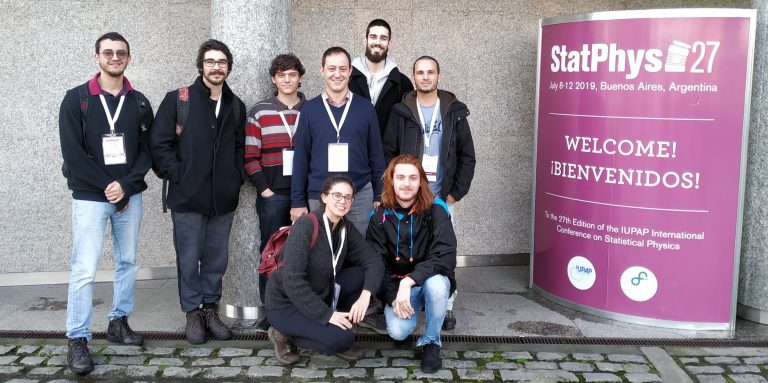
\includegraphics[scale=0.3]{Imagens/group.jpg}
  \end{figure}



\end{frame}

\begin{frame}
  \frametitle{My masters project}
  \begin{itemize}
  \item I'm studying a model called GEM-$\alpha$ that could model some colloidal suspensions and ultracold atoms;
  \item And that forms some special patterns know as cluster cristals.
  \end{itemize}
  \begin{figure}
    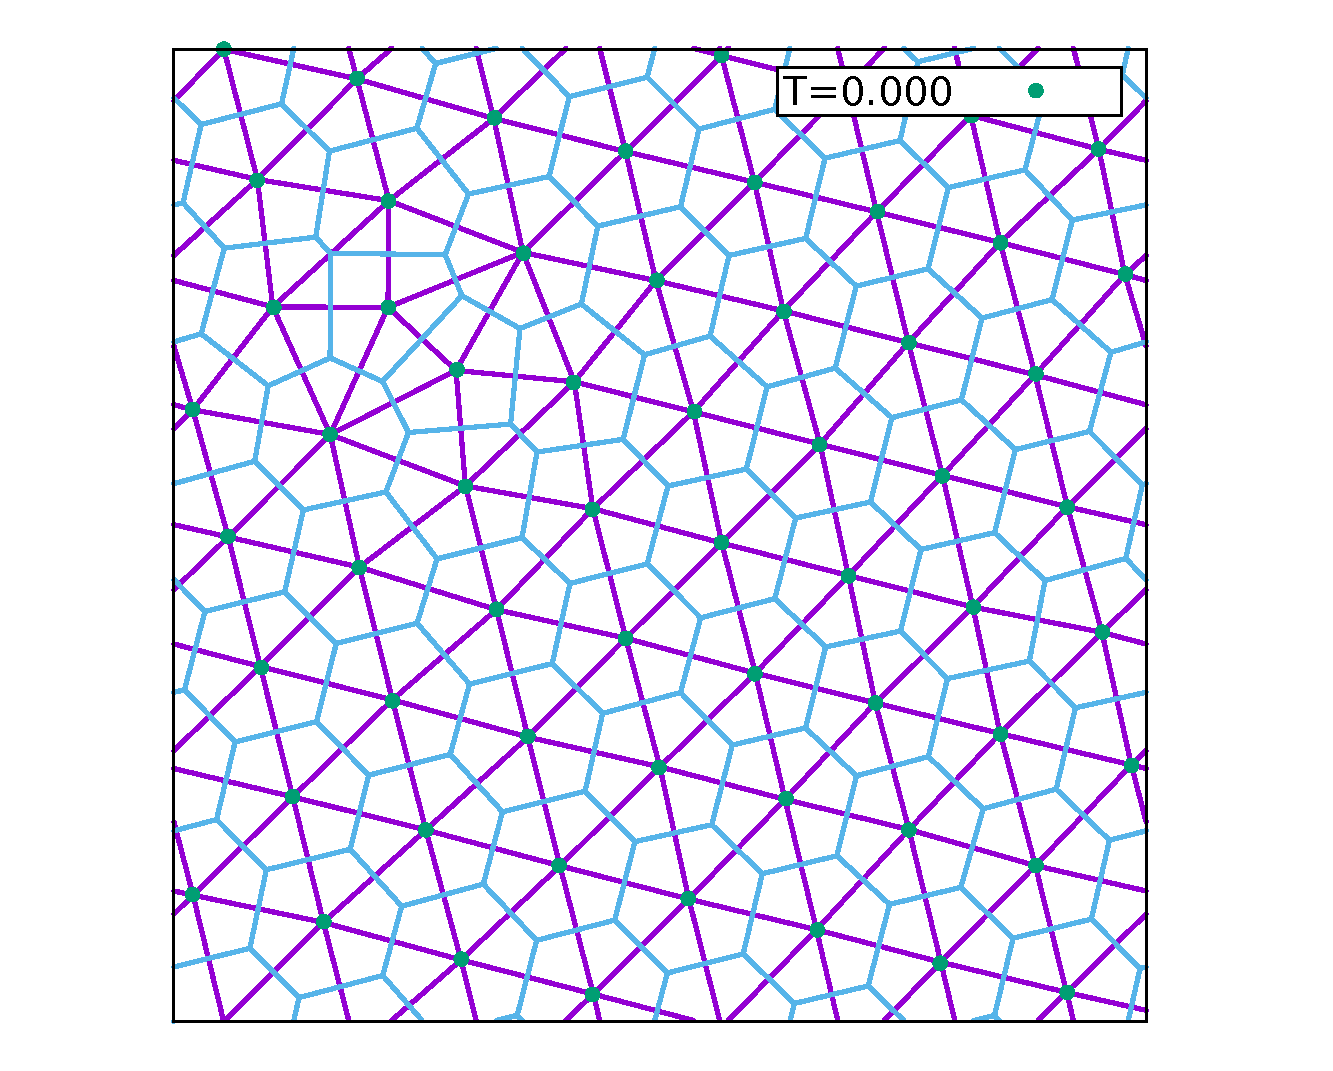
\includegraphics[scale=0.17]{Imagens/T0000.pdf}
    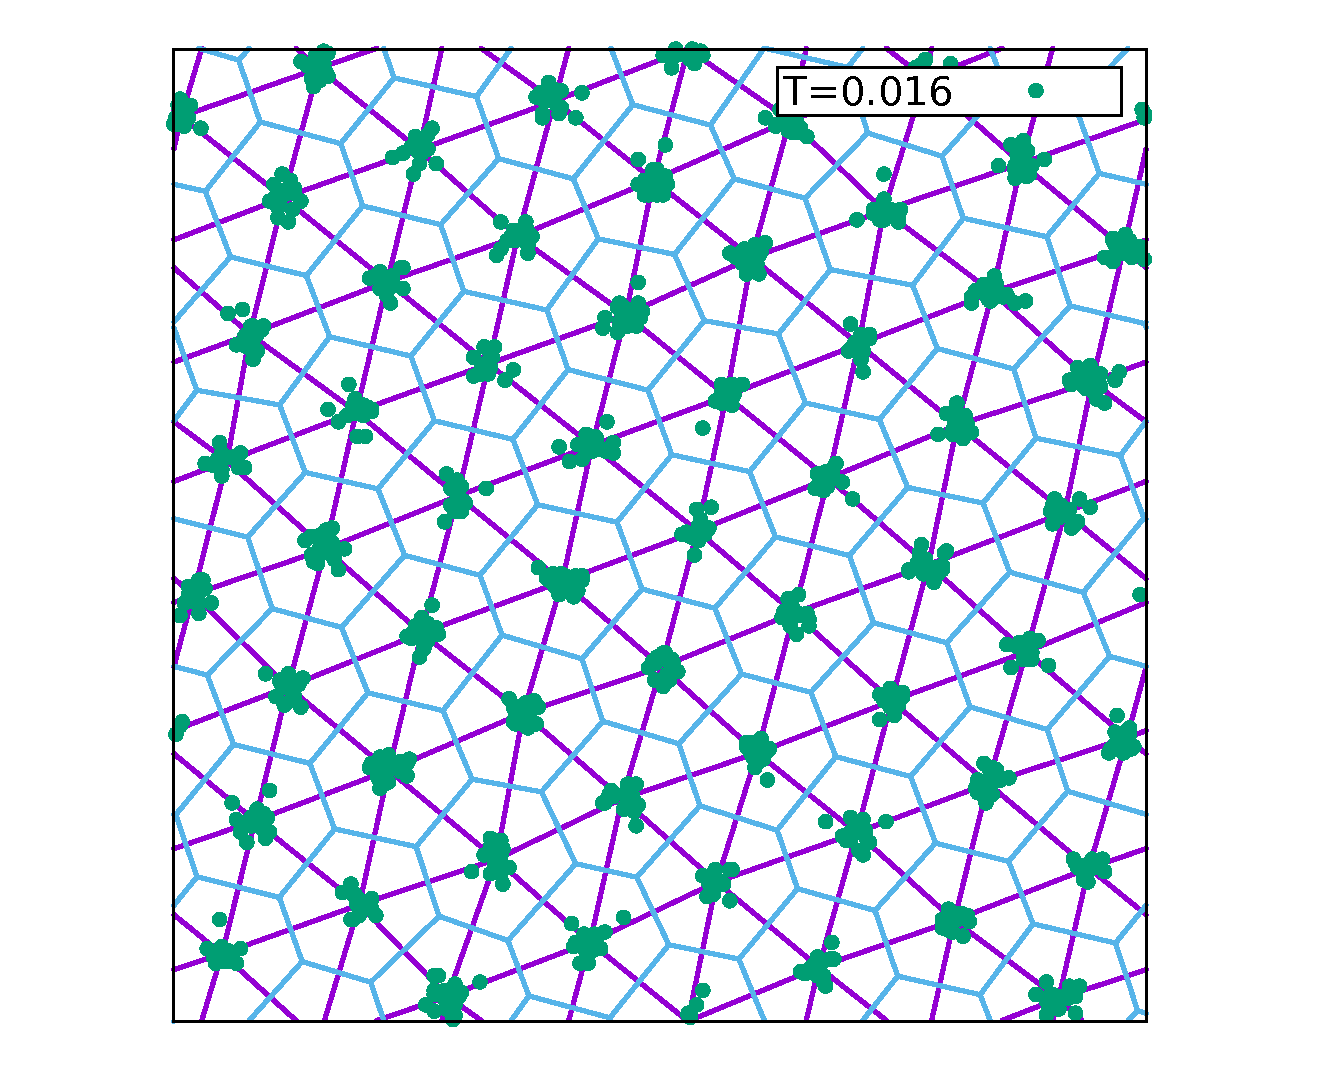
\includegraphics[scale=0.17]{Imagens/T0016.pdf}
    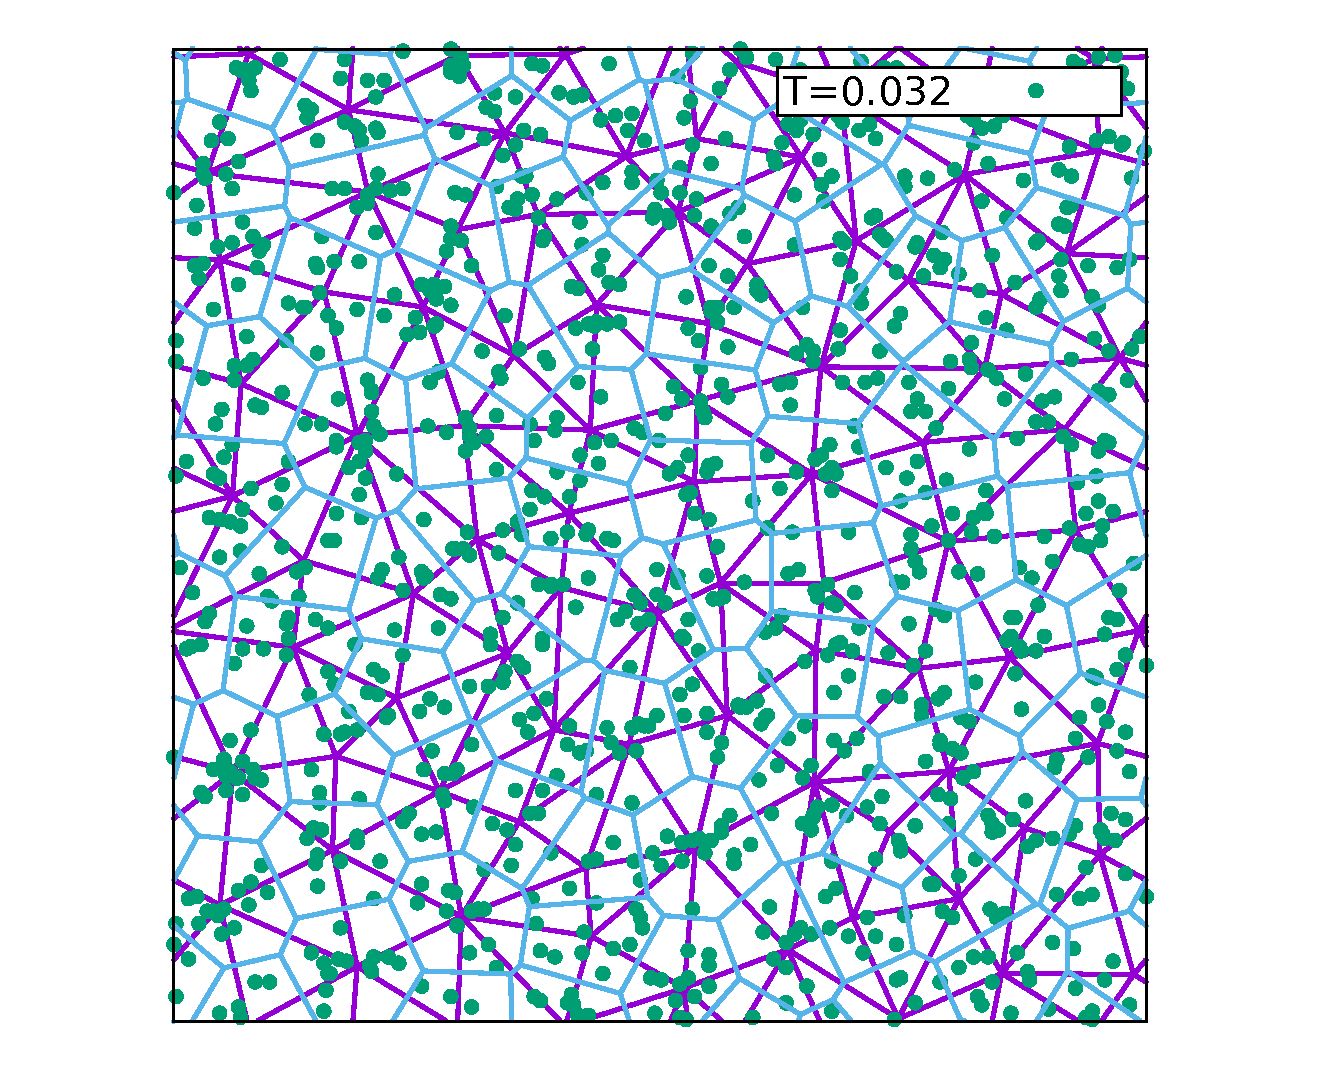
\includegraphics[scale=0.17]{Imagens/T0032.pdf}
  \end{figure}
\end{frame}

\begin{frame}
  \frametitle{What is my problem?}
  \begin{itemize}
  \item We generally want to get out of metastable states;
  \item Equilibrate simulation in various temperatures;
  \item We don't want to waste time doing bad annealing that may not be in a equilibrium state.
  \end{itemize}

  \begin{center}
    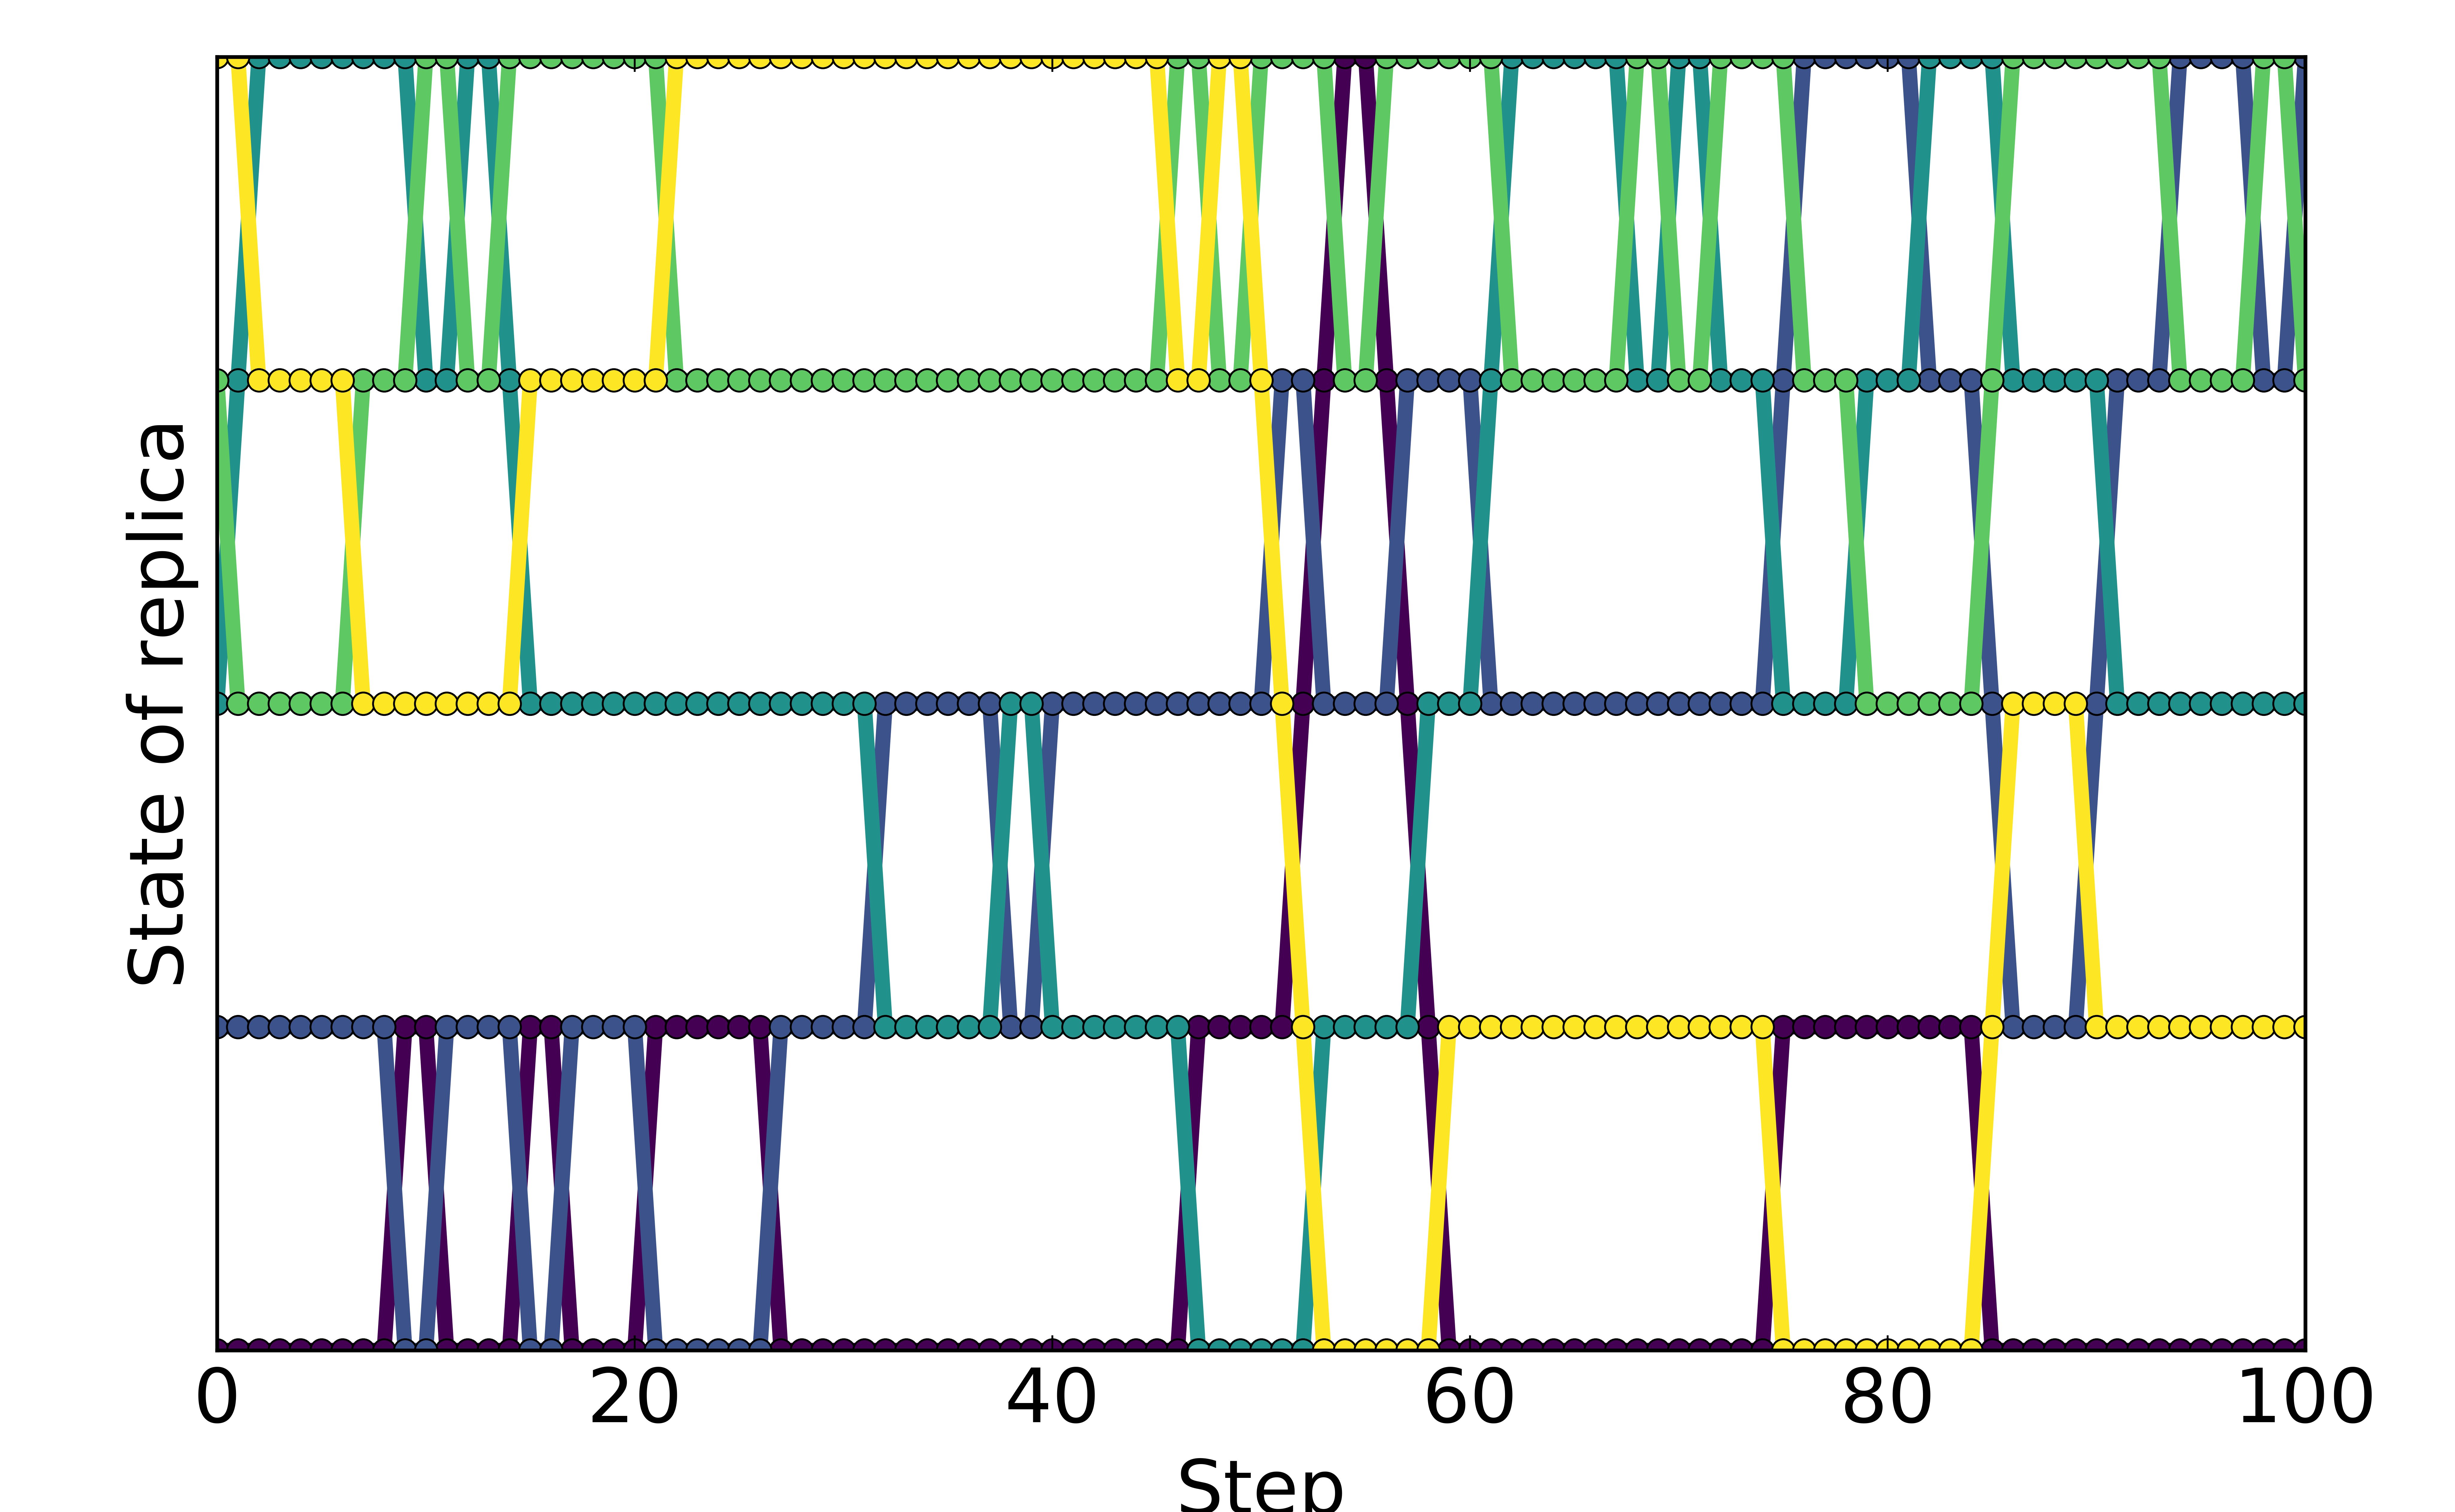
\includegraphics[width=0.5\textwidth]{Imagens/pt.png}
  \end{center}

  \begin{itemize}
  \item So, to solve all that problems we can use the \textbf{parallel tempering} technique;
  \end{itemize}
\end{frame}

\begin{frame}
  \frametitle{Parallel Tempering}
  \begin{itemize}
  \item In my simulations, the temperature is a fixed variable and energy could flutuate $\rightarrow$ Canonical ensemble;
  \item So if we look at the energy histograms, we will see a overlap between differents temperatures;
    \begin{center}
      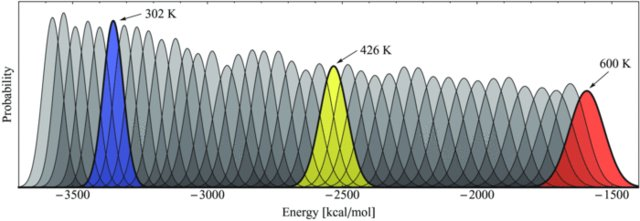
\includegraphics[scale=0.3]{Imagens/histos.jpg}
    \end{center}
  \item This overlap could be interpreted as the probability of the configuration at this temperature could be at the other temperature;
  \item We can calculate the total probability of two configurations have been changed using the Boltzmann weight;
  \end{itemize}

  $$ p(i,j)=min\left(1,\dfrac{e^{-\beta_i E_j-\beta_j E_i}}{e^{-\beta_i E_i-\beta_j E_j}}\right)=min\left(1,e^{(E_i-E_j)(\beta_i-\beta_j)}\right) $$
\end{frame}

\begin{frame}
  \frametitle{How can we parallelize?}

  \begin{itemize}
  \item Just a task farming, so...
  \end{itemize}

  \begin{figure}[h!]
    \centering
    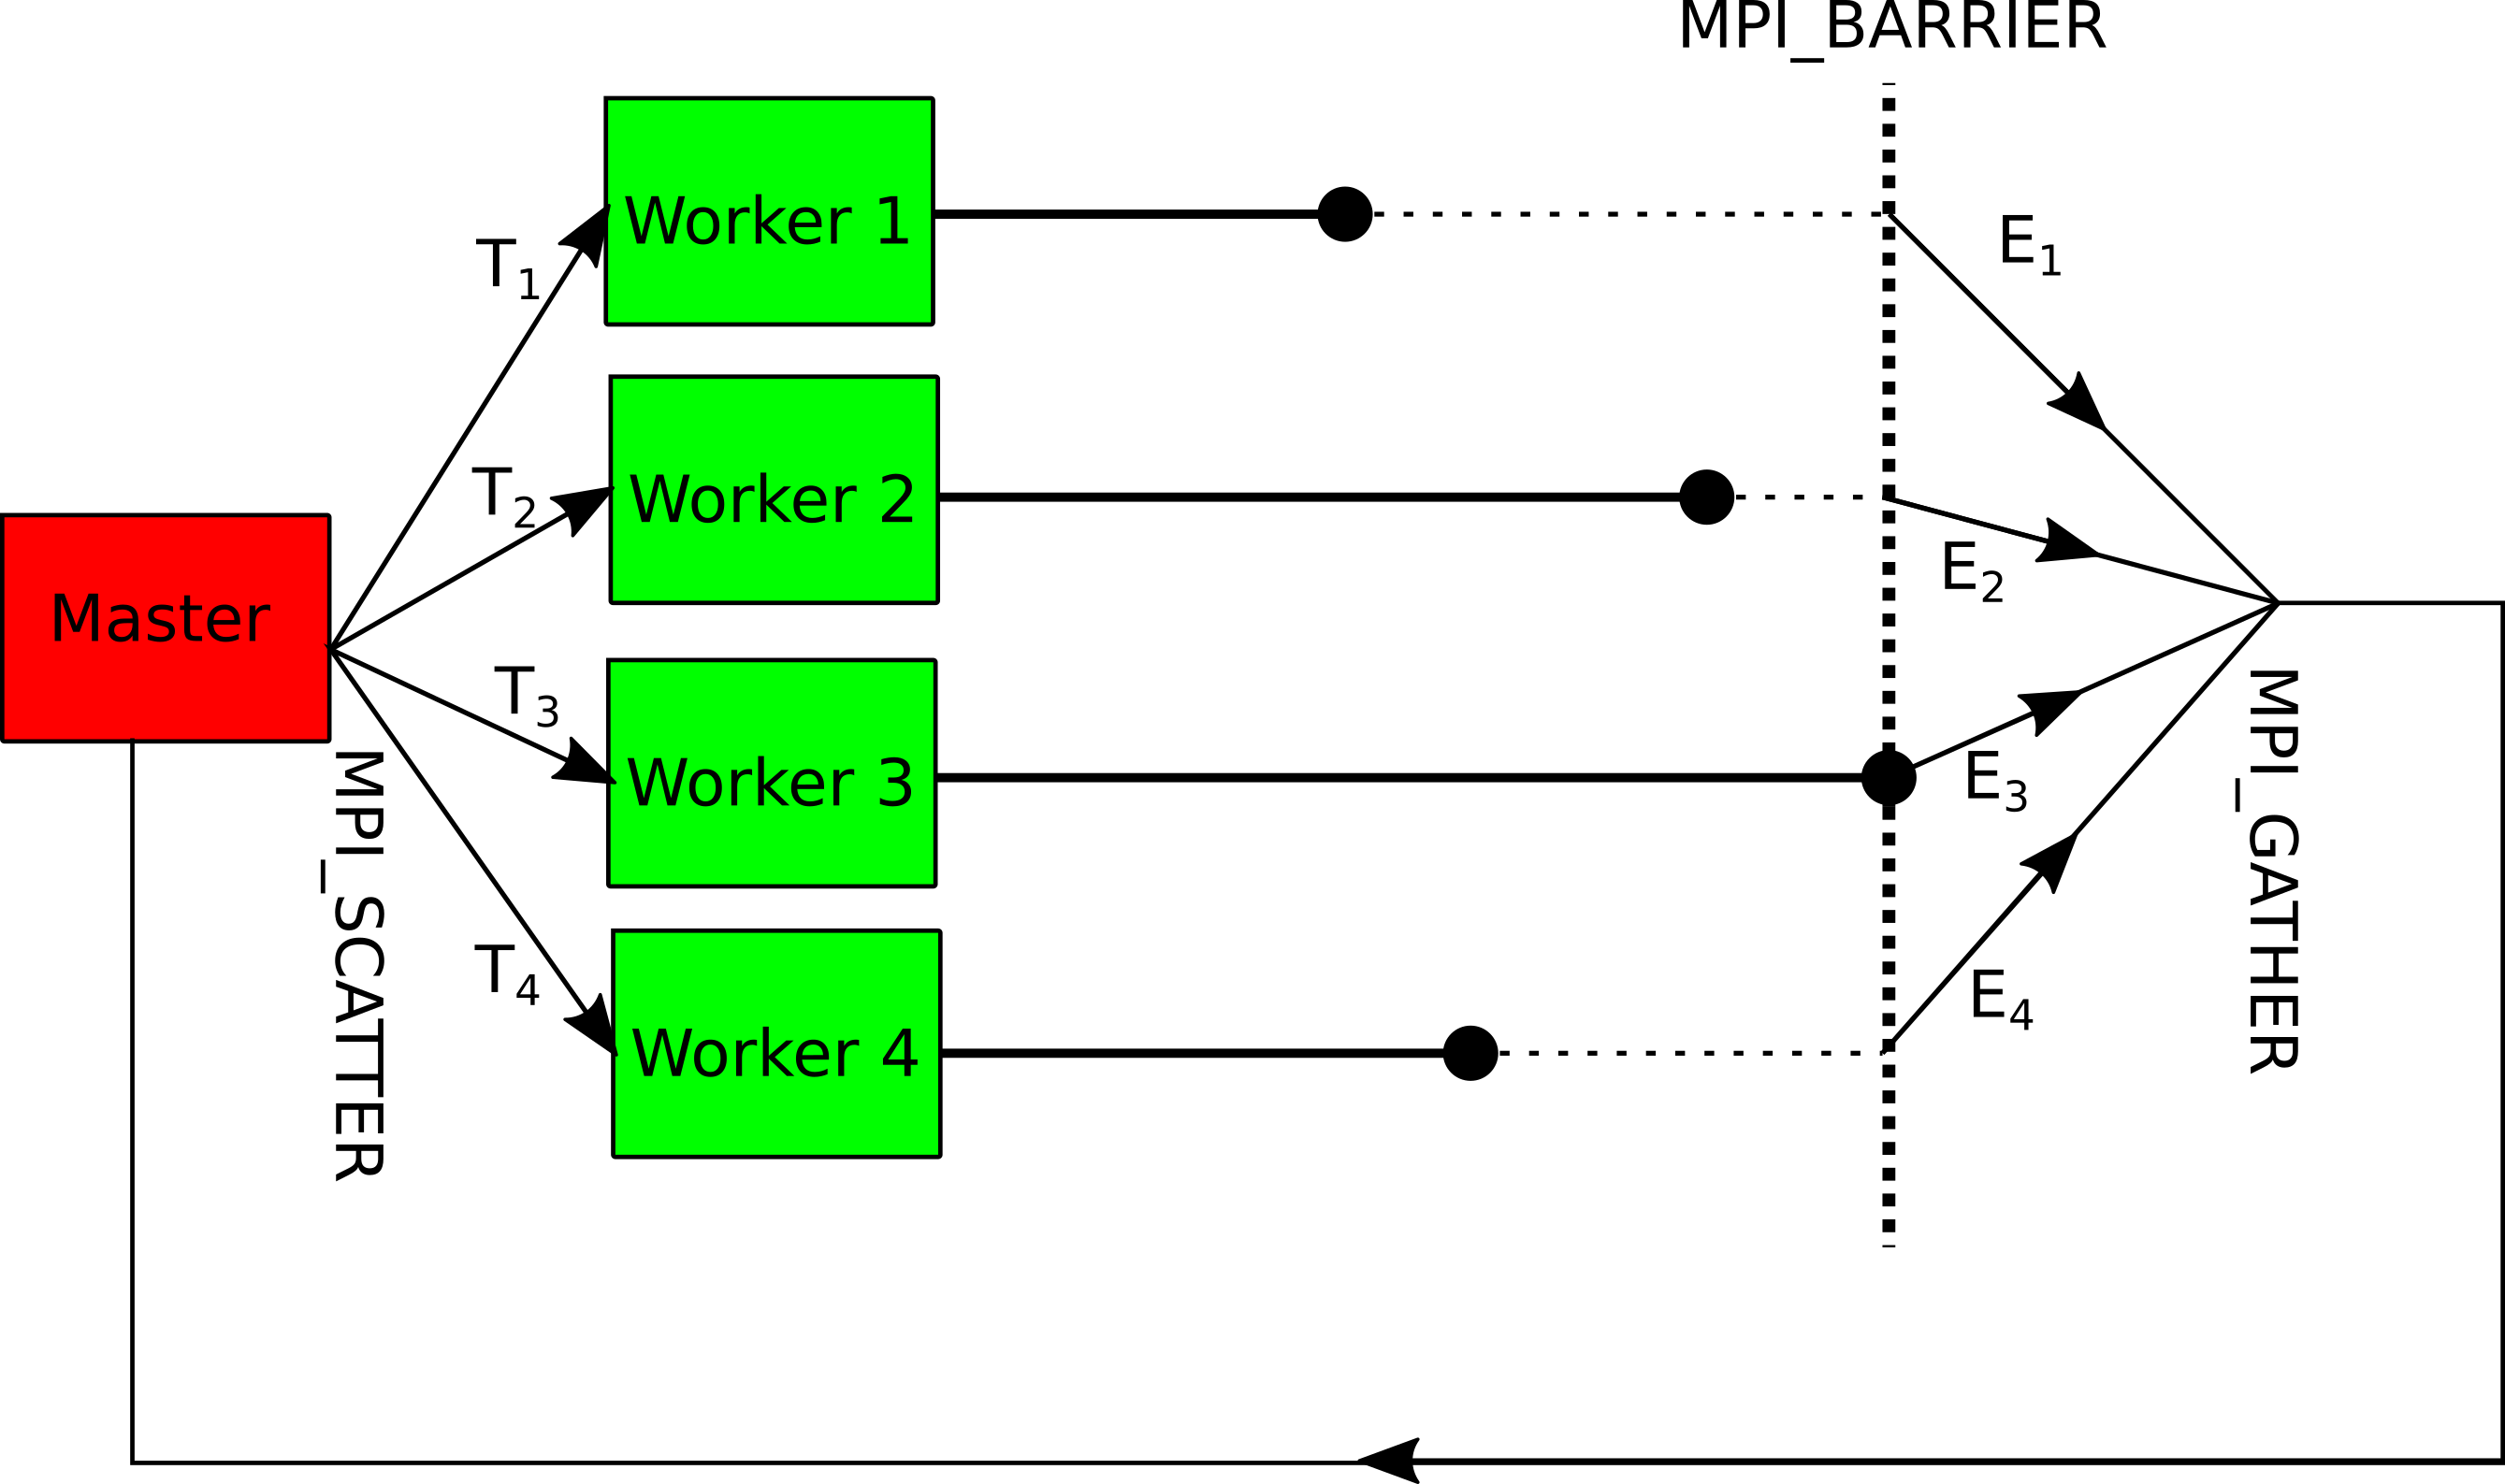
\includegraphics[scale=0.6]{Imagens/taskFarm.png}
  \end{figure}
\end{frame}

\begin{frame}[fragile]
  \begin{tiny}
\begin{verbatim}
  for(trials=0; trials<300; trials++){
    MPI_Barrier(MPI_COMM_WORLD);
    MPI_Scatter(allT, 1, MPI_DOUBLE, &T, 1, MPI_DOUBLE, 0, comm);

    // update all the ensembles in the same time, one per thread
    for(k=0; k<Kmax; k++){ 
     update(x, y, T); 
    }

    // wait all the evolutions finish
    MPI_Barrier(MPI_COMM_WORLD);

    // measure the energy of each ensemble and send to master
    E = ener(x, y);

    MPI_Gather(&E, 1, MPI_DOUBLE, allE, 1, MPI_DOUBLE, 0, comm);
    
    // decides who changes temperature with who
    if(pt==0){
      for(i=0; i<PT-1; i++){
        delta=-(1./allT[confT[i+1]]-1./allT[confT[i]])*(allE[confT[i+1]]-allE[confT[i]]);
        if(delta<0 || FRANDOM<exp(-delta)){
          aux=confT[i];
          confT[i]=confT[i+1];
          confT[i+1]=aux;

          aux=allT[i+1];
          allT[i+1]=allT[i];
          allT[i]=aux;
        }
      }
    }
  }
\end{verbatim}
  \end{tiny}
\end{frame}

\begin{frame}
  \frametitle{Load Balance}

  \begin{itemize}
  \item Okay, so now we have a truly \textbf{parallel} tempering, running at different cores;
  \item But to running Ntemps temperatures we need Ntemps cores;
  \item So, when we have a small cluster, how the ours: 14 quad-core nodes = 48 processing elements, we can just run 48 temperatures;
  \item How to simulate more temperatures in this enviroment without losing much time with one process and almost anything with the other?
  \end{itemize}
\end{frame}


\begin{frame}
  \frametitle{Load Balance}

  \begin{figure}[h!]
    \centering
    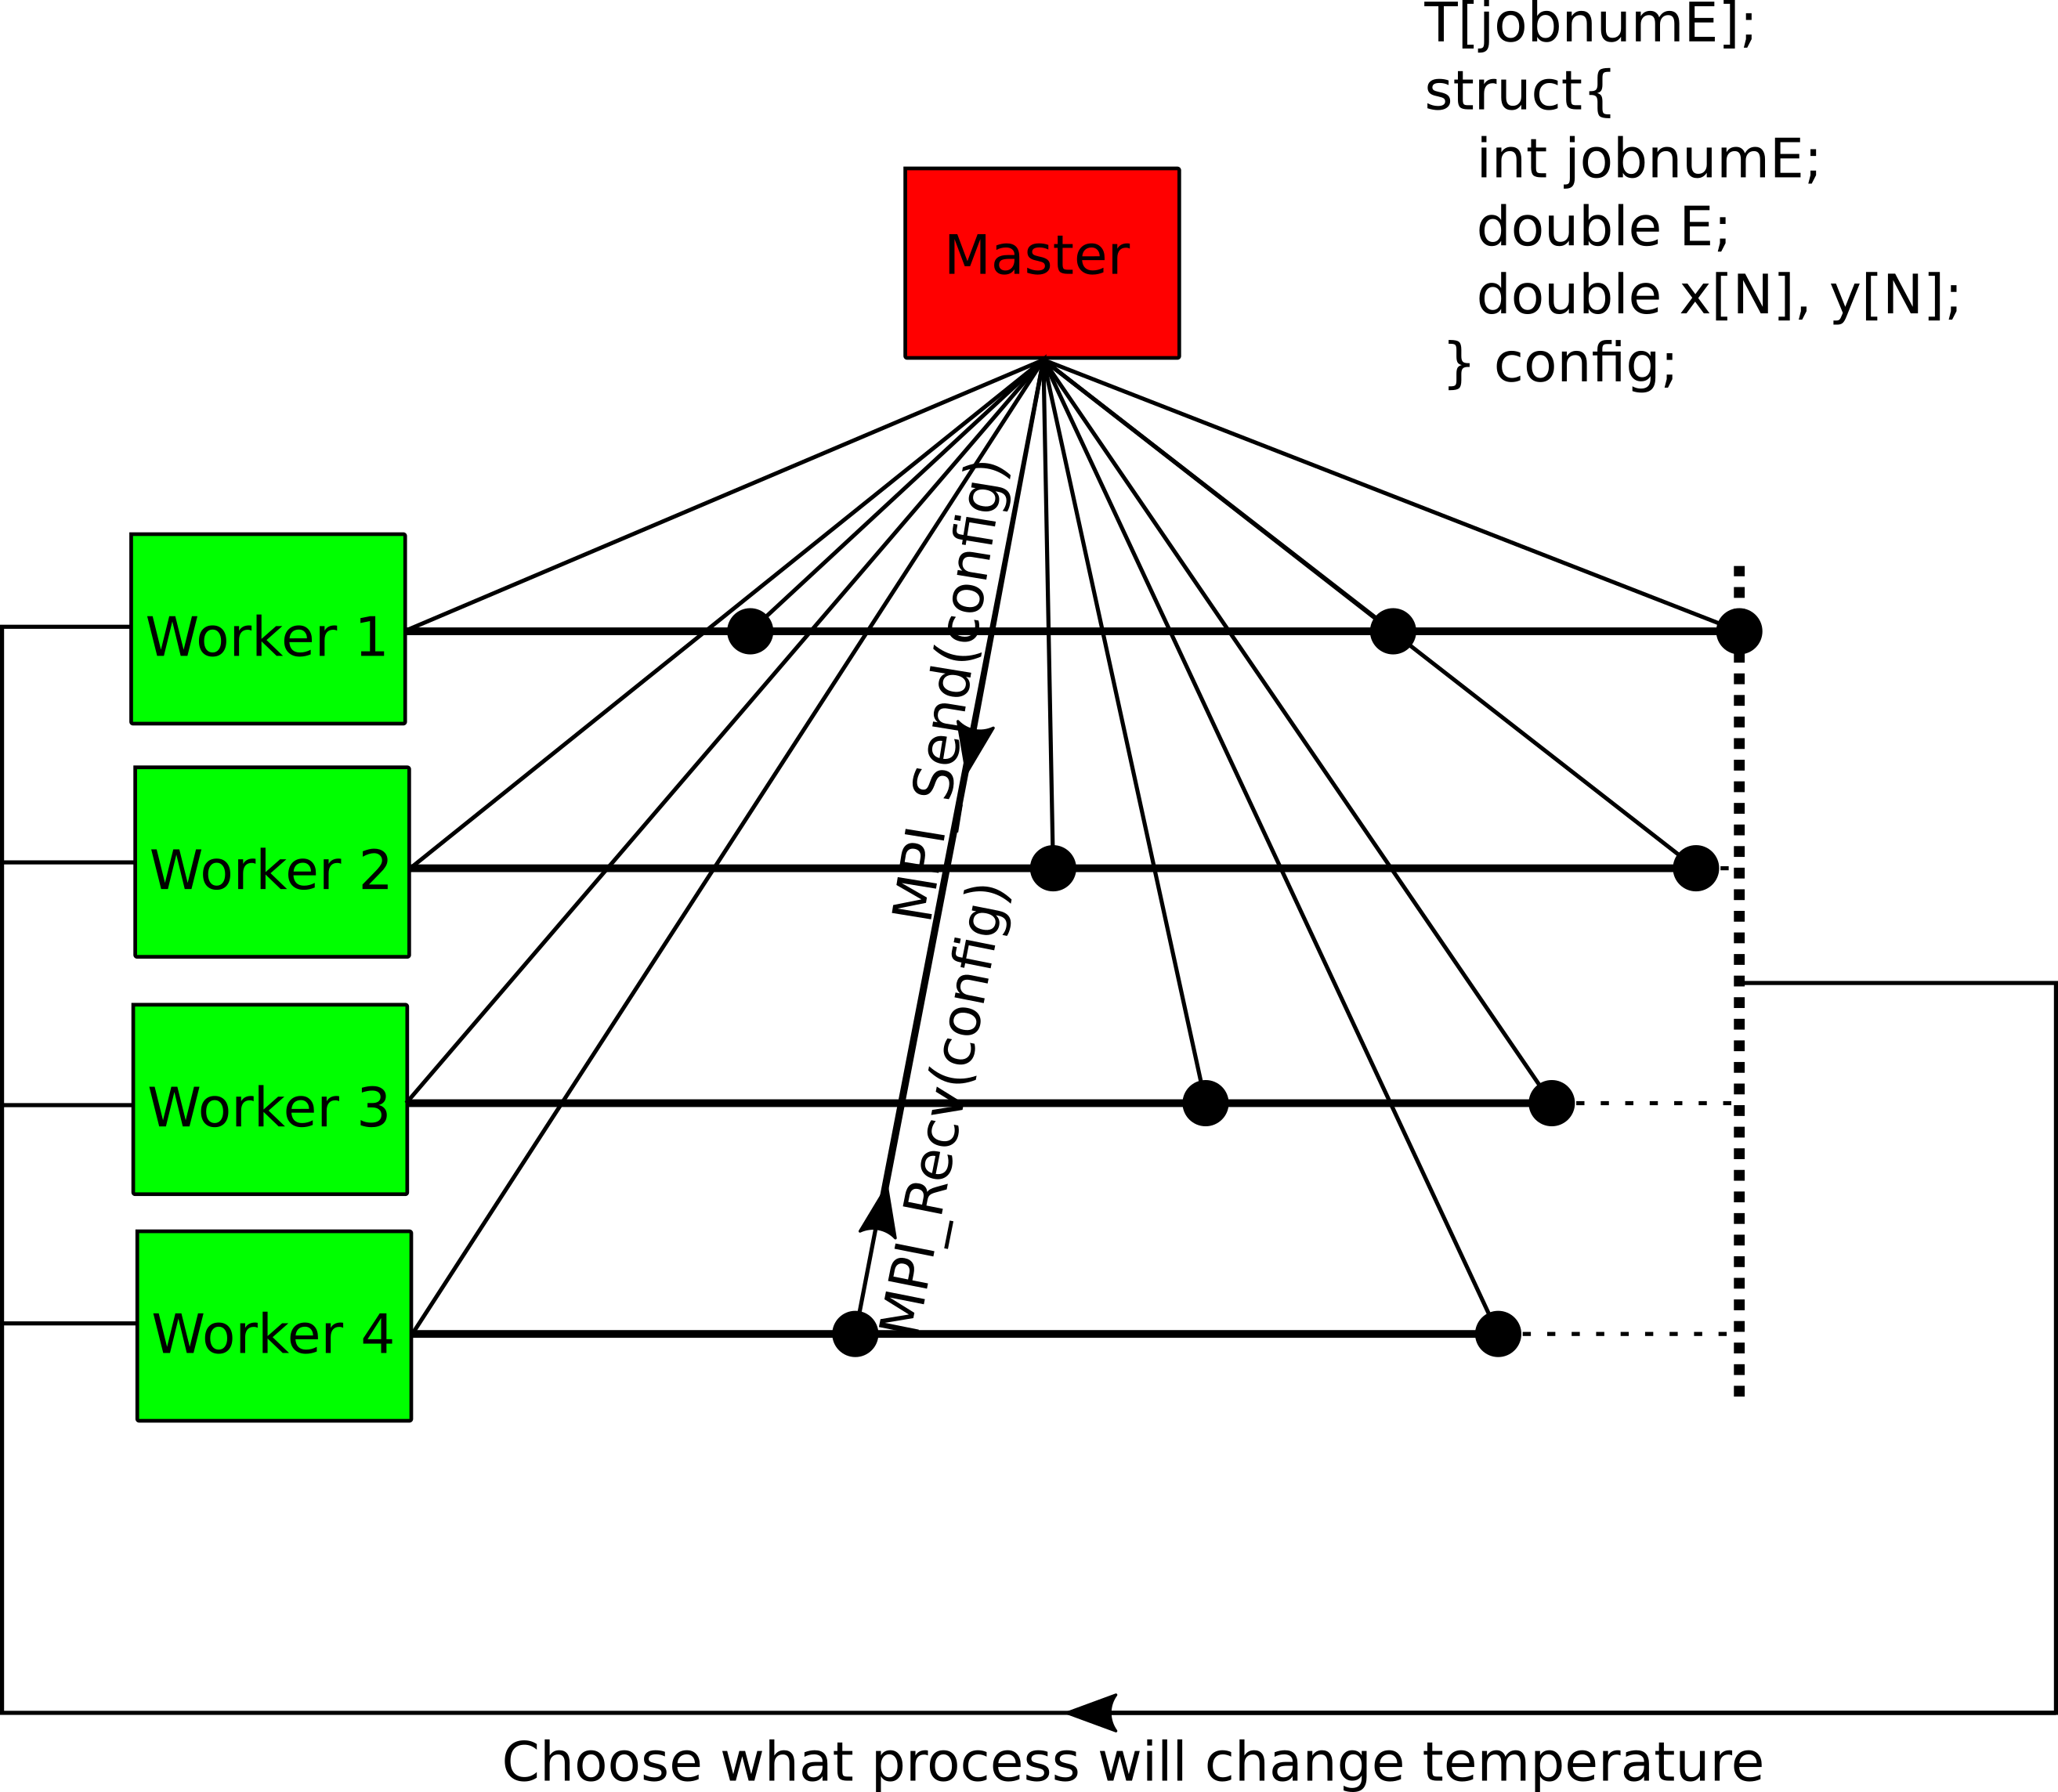
\includegraphics[scale=0.6]{Imagens/loadBalance.png}
  \end{figure}
\end{frame}

\begin{frame}[fragile]
  \begin{tiny}
    \begin{columns}
      \begin{column}{0.5\textwidth}
\begin{verbatim}
// master process
if(!rank){
  // initiates sending one process to each rank
  for(jobnum=0; jobnum<Nranks-1; jobnum++){
    configs[jobnum].jobnumE = jobnum;
    MPI_Send(&configs[jobnum], 1, MPI_Config,\
             jobnum+1, flag, comm);
  }
  
  // still has jobs to do
  for(jobnum=Nranks-1; jobnum<Ntemps; jobnum++){
    // wait for any rank finish to send another job
    MPI_Recv(&jobnumE, 1, MPI_INT,\
             MPI_ANY_SOURCE, 0, comm, &stat);
    MPI_Recv(&configs[jobnumE], 1, MPI_Config,\
             stat.MPI_SOURCE, 1, comm,\
             MPI_STATUS_IGNORE);

    configs[jobnum].jobnumE = jobnum;
    MPI_Send(&configs[jobnum], 1, MPI_Config,\
             stat.MPI_SOURCE, 0, comm);
  }

  // for the last ones just recv energies and\
     send a -1 to says that its over
  for(dest=1; dest<Nranks; dest++){
    MPI_Recv(&jobnumE, 1, MPI_INT,\
             MPI_ANY_SOURCE, 0, comm, &stat);
    MPI_Recv(&configs[jobnumE], 1, MPI_Config,\
             stat.MPI_SOURCE, 1, comm,\
             MPI_STATUS_IGNORE);
	
    configs[jobnum].jobnumE = -1;
    MPI_Send(&configs[jobnum], 1, MPI_Config,\
             stat.MPI_SOURCE, 0, comm);
  }
}
\end{verbatim}
      \end{column}
      \begin{column}{0.5\textwidth}
\begin{verbatim}
// worker process
else{
  while(1){
    MPI_Recv(&configs[0], 1, MPI_Config,\
             0, 0, comm, MPI_STATUS_IGNORE);
    if(configs[0].jobnumE>=0) {
      // update Nranks ensembles at the same time,\
         one per rank
      for(k=0; k<Kmax; k++){
        update(configs[0].x, configs[0].y,\
               allT[configs[0].jobnumE]);
      }
	
      // measure the energy and send back to the root
      configs[0].E=ener(configs[0].x, configs[0].y);
      MPI_Send(&configs[0].jobnumE, 1, MPI_INT,\
               0, 0, comm);
      MPI_Send(&configs[0], 1, MPI_Config,\
               0, 1, comm);
    }
    else{
      break;
    }
  }
}
\end{verbatim}
      \end{column}
    \end{columns}
  \end{tiny}
\end{frame}

\begin{frame}
  \frametitle{Results}

  \centering
  \begin{columns}
    \begin{column}{0.5\textwidth}
      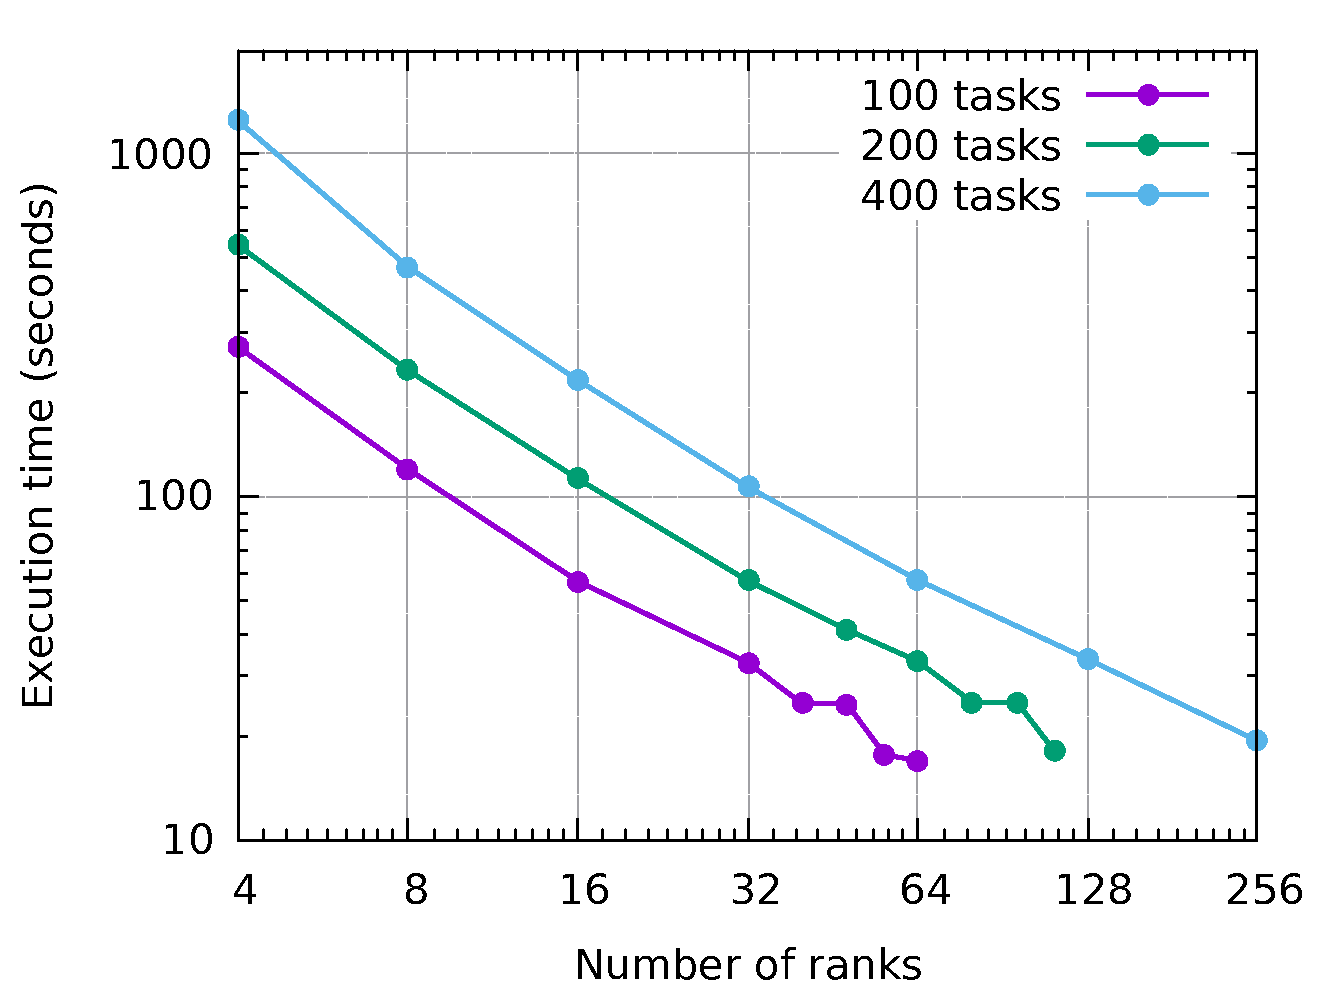
\includegraphics[width=\textwidth]{Imagens/exectime.pdf}
    \end{column}
    \begin{column}{0.5\textwidth}
      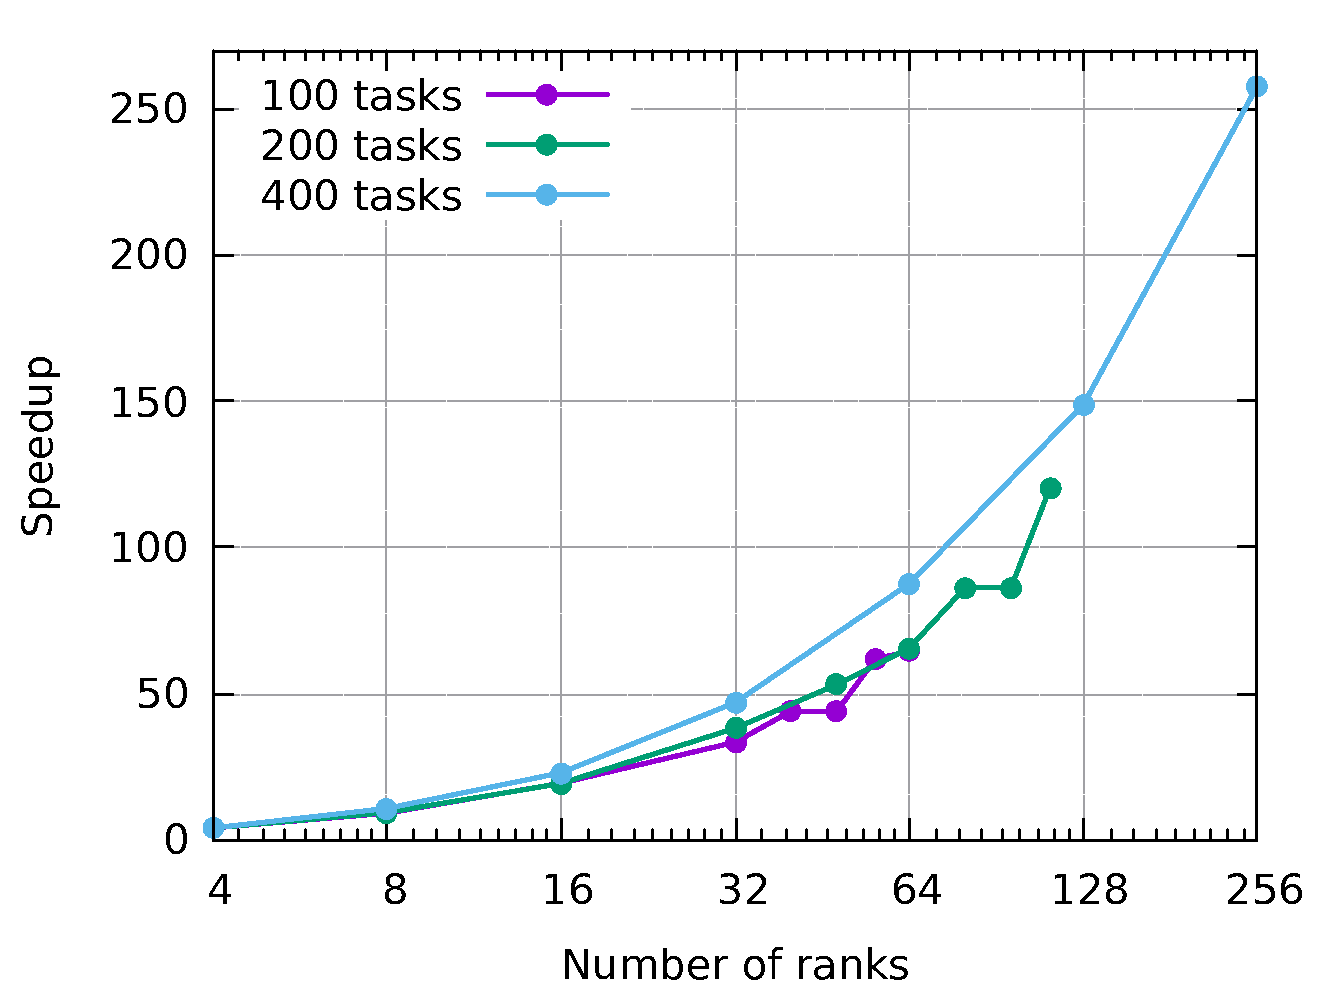
\includegraphics[width=\textwidth]{Imagens/speedup.pdf}
    \end{column}
  \end{columns}
  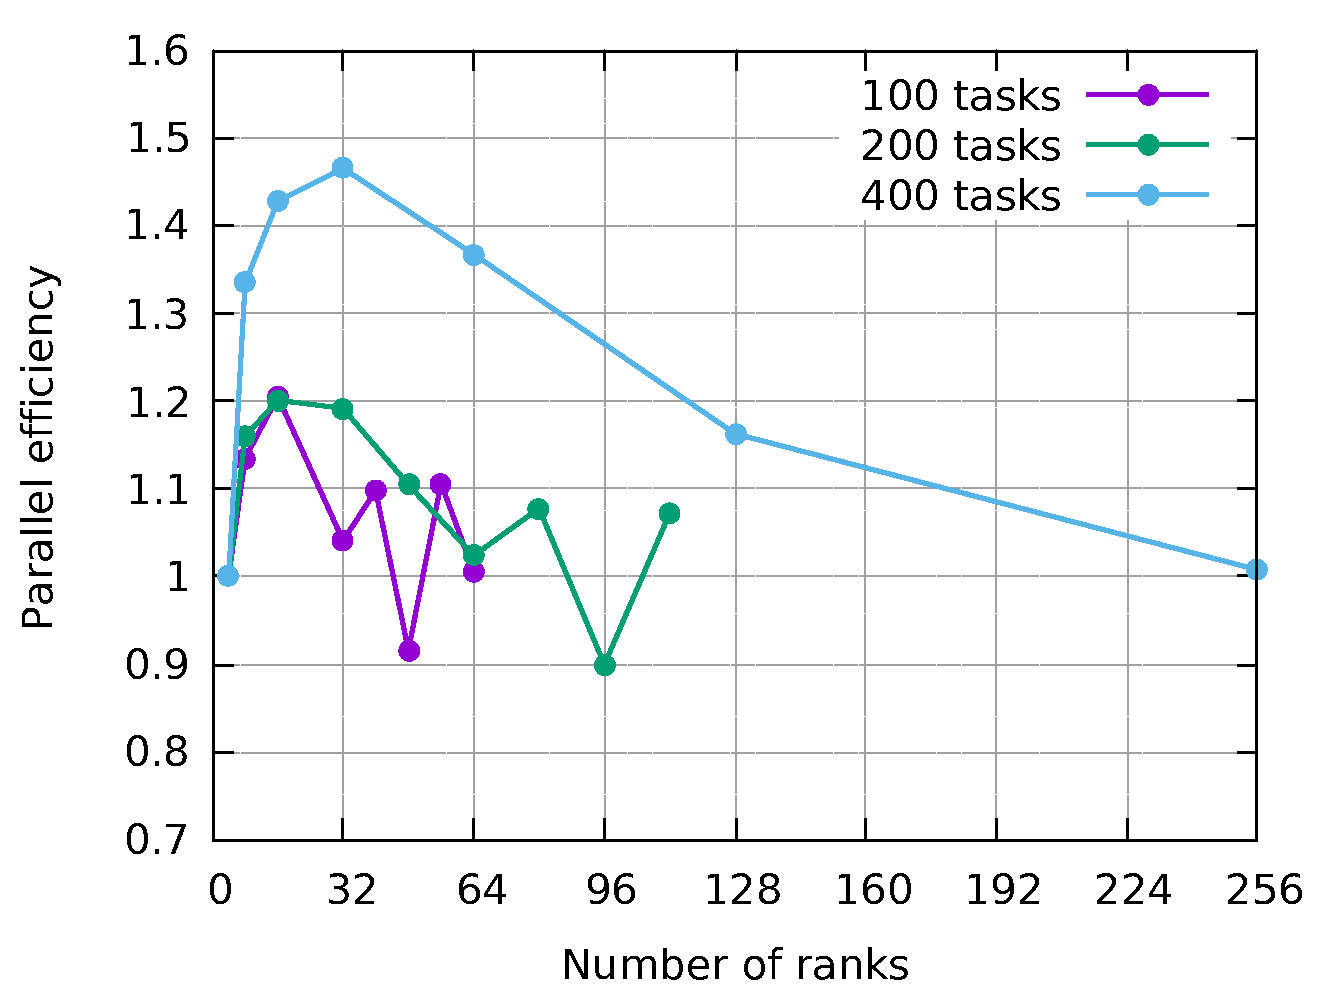
\includegraphics[width=0.5\textwidth]{Imagens/efficiency.pdf}
\end{frame}

\end{document}